\section{Vectorization of data}\label{vectorization}\marginnote{GM}
\begin{text}
After the first attempt to make learning more efficient through parallelization, without any effect, we thought about vectorization of the data. For this we take a look at the encryption of data. The CKKS library gives us two options for the encryption. We can encrypt the data as vectors or as tensors. If we encrypt the input as tensors we can encrypt whole matrices in one step.
\end{text}

\subsection{Space requirements}\marginnote{GM}
\begin{text}
The first drawback of our idea for learning on encrypted data was the required space for the encrypted data. So we take a closer look on this topic. We used several matrices as inputs and encrypt them all with the same CKKS context that we have used so far. In the table of figure \ref{fig:baseline} we can see how many megabyte are used for the encryption of $m$ data points with dimension $n$ where we encrypted each single data point with one CKKS vector. These results are our baseline to see if we can find better ways to encrypt a whole data set.
\end{text}

\begin{figure}[ht]
\centering
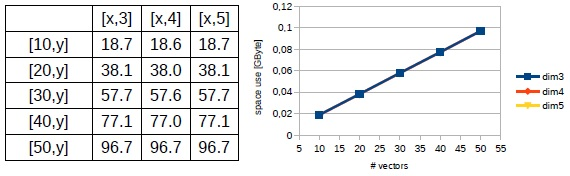
\includegraphics[width=1\linewidth]{images/baseline.jpg}
\caption{Space requirements of encrypted $[m\times n]$-matrices as vectors row by row in megabyte.}
\label{fig:baseline}
\end{figure} 

\begin{text}
With the graph of figure \ref{fig:baseline} we can easily see that the dependency on dimension of the data points is not measurable for our small dimensions and that the encryption of multi vectors is linear. \newline
\indent Next, we measure the space requirements of CKKS tensors. We use the same context and the input arrays like before but now we encrypt the whole $m$ data points with dimension $n$ with only one CKKS tensor. The idea is that the CKKS scheme can encrypt multiple data points more efficient as a CKKS tensor by its own than we do before. In the table of figure \ref{fig:tensor} we can see how many megabyte are used for the encryption.
\end{text}

\begin{figure}[ht]
\centering
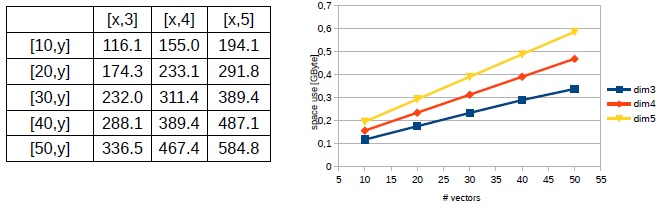
\includegraphics[width=1\linewidth]{images/tensor.jpg}
\caption{Space requirements of encrypted $[m\times n]$-matrices as one tensor in megabyte.}
\label{fig:tensor}
\end{figure} 

\begin{text}
With the graph of figure \ref{fig:tensor} we can see that the dimension of the data points has an impact. Higher dimension use more space than lower dimension and over all the space requirements are much more than the encryption row by row. So the encryption as a CKKS tensor doesn't solve the space requirement problem we have. \newline
From the results of the measurements of the baseline that the dependency on dimension of the data points is not measurable for our small dimensions we try to find a limit where we see a dependency on dimension. For this we flatten the matrix in such a way that we have only a vector with a dimension of m times n.We encrypt this vector with the same context like before.
\end{text}

\begin{figure}[ht]
\centering
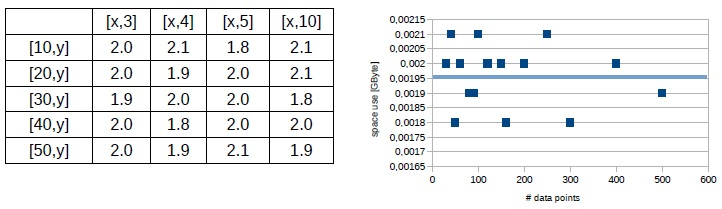
\includegraphics[width=1\linewidth]{images/flatten.jpg}
\caption{Space requirements of encrypted flatten $[m\times n]$-matrices as vector in megabyte.}
\label{fig:flatten}
\end{figure} 

\begin{text}
In figure \ref{fig:flatten} we can see that the flatten matrix use nearly the same space for each vector independent of the dimension at least for our data range. So we can handle the high space requirement of our algorithm if we use flatten matrices as an input and we can find a way to calculate with such a flatten matrix.
\end{text}

\subsection{Calculation with vectorized data}\marginnote{GM}
\begin{text}
Let's assume that all users stores their encrypted data points as a struc where you know the dimension $n$ of the data points and the number $m$ of data points that are encrypted. Maybe you need the context how the data points are encrypted and at least the encrypted data points as a vector. Figure \ref{fig:vec} a) shows an example of such an vectors. In the example $x_{m,1}$ and $x_{m,2}$ are the coordinates of the 2-dimensional data points, $b_m$ is the bias that is usually set to 1 and $y_m$ is the expected output. With this struc we are going to create another vector, a weight vector. The size of the weight vector is the same size like the data vector. Figure \ref{fig:vec} b) shows an example of such a weight vector. In the example we have a sub sequence of two weights $w_1$ and $w_2$ to weight the coordinates, another weight $w_b$ to wight the bias followed by a $1$. This sub sequence is repeated $m$ times in the whole weight vector. \newline

\begin{figure}[ht]
    \centering
    \begin{tabular}{c|c|c|c|c|c|c|c|c|c|c|c|c|c}
        \cline{2-13}
        a) & $x_{1,1}$ & $x_{1,2}$ & $b_{1}$ & $y_{1}$ & $x_{2,1}$ & $x_{2,2}$ & $b_{2}$ & $y_{2}$ & $x_{3,1}$ & $x_{3,2}$ & $b_{3}$ & $y_{3}$ & $\dots$  \\
        \cline{2-13}
        \noalign{\medskip}
        \cline{2-13}
        b) & $w_1$ & $w_2$ & $w_b$ & $1$ & $w_1$ & $w_2$ & $w_b$ & $1$ & $w_1$ & $w_2$ & $w_b$ & $1$ & $\dots$  \\
        \cline{2-13}
    \end{tabular}
    \caption{a) Encrypted data point vector. b) Weight vector}
    \label{fig:vec}
\end{figure}

After the encryption of the weight vector we can replace the for loop to calculate $\Delta$w in our algorithm \ref{threadfunction} with simple vector arithmetic. We multiply the encrypted data point vector point-wise with the weight vector. The resulting vector together with the data point vector includes all values we need to calculate $\Delta$w. Figure \ref{fig:resvec} illustrates this calculation. \newline

\begin{figure}[ht]
    \centering
    \begin{tabular}{|c|c|c|c|c|c|c|c|c|c|c|c|c}
        \cline{1-12}
        $x_{1,1}$ & $x_{1,2}$ & $b_{1}$ & $y_{1}$ & $x_{2,1}$ & $x_{2,2}$ & $b_{2}$ & $y_{2}$ & $x_{3,1}$ & $x_{3,2}$ & $b_{3}$ & $y_{3}$ & $\dots$  \\
        \cline{1-12}
        \noalign{\smallskip}
        \multicolumn{13}{c}{point-wise multiplication} \\
        \noalign{\smallskip}
        \cline{1-12}
        $w_1$ & $w_2$ & $w_b$ & $1$ & $w_1$ & $w_2$ & $w_b$ & $1$ & $w_1$ & $w_2$ & $w_b$ & $1$ & $\dots$  \\
        \cline{1-12}
        \noalign{\smallskip}
        \multicolumn{13}{c}{$=$} \\
        \noalign{\smallskip}
        \cline{1-12}
        $w_1 x_{1,1}$ & $w_2 x_{1,2}$ & $w_b b_{1}$ & $y_{1}$ & $w_1 x_{2,1}$ & $w_2 x_{2,2}$ & $w_b b_{2}$ & $y_{2}$ & $w_1 x_{3,1}$ & $w_2 x_{3,2}$ & $w_b b_{3}$ & $y_{3}$ & $\dots$  \\
        \cline{1-12}    
    \end{tabular}
    \caption{Calculation of the resulting vector}
    \label{fig:resvec}
\end{figure}

To calculate $\Delta$w we need the output, the expected output and the input. With an encrypted selection vector we are able to choose parts from the data point and resulting vector we need. Figure \ref{fig:chovec} shows an example where we select the parts of the resulting vector that we need to approximate the output of the neuron with the first data point as input.

\begin{figure}[ht]
    \centering
    \begin{tabular}{|c|c|c|c|c|c|c|c|c|c|c|c|c}
        \cline{1-12}
        $w_1 x_{1,1}$ & $w_2 x_{1,2}$ & $w_b b_{1}$ & $y_{1}$ & $w_1 x_{2,1}$ & $w_2 x_{2,2}$ & $w_b b_{2}$ & $y_{2}$ & $w_1 x_{3,1}$ & $w_2 x_{3,2}$ & $w_b b_{3}$ & $y_{3}$ & $\dots$  \\
        \cline{1-12}
        \noalign{\smallskip}
        \multicolumn{13}{c}{dot product} \\
        \noalign{\smallskip}
        \cline{1-12}
        $1$ & $1$ & $1$ & $0$ & $0$ & $0$ & $0$ & $0$ & $0$ & $0$ & $0$ & $0$ & $\dots$  \\
        \cline{1-12}
        \noalign{\smallskip}
        \multicolumn{13}{c}{$=$} \\
        \noalign{\smallskip}
        \multicolumn{13}{c}{$w_1 x_{1,1} + w_2 x_{1,2} + w_b b_{1}$} \\
    \end{tabular}
    \caption{Selection of the results for the first data point as input.}
    \label{fig:chovec}
\end{figure}

To the result of the selection in figure \ref{fig:chovec} we can now apply the approximation of the sigmoid function to get the output. With a different selection vector we can choose the corresponding expected output like before. With another selection vector we need to select the corresponding data point. Now we are able to use the calculation of $\Delta$w from our algorithm \ref{code:pseudocode}. \newline
If we use the selection vectors for each data point we can run our algorithm for learning with encrypted vectors. But to get a speed up by using vectors we need to use matrix multiplications instead of vector multiplications because otherwise we replace one for loop with another. But for now matrix multiplications in the CKKS scheme is still missing.
\end{text}